\section{Experimental details}\label{sec:experimental_details}

In this section, we give further experimental details including architectures, hyperparameters, and implementation details. All models and experiments are implemented in Tensorflow. The code is publicly available on the project repo along with detailed experimental logs and instructions for reproducing our results.

\subsection{Discriminative tasks (\Cref{ssec:experiments_discriminative})}


\subsubsection{Pairwise Order}
Each model in this experiment has the following form $\texttt{input} \to \{ \cdot \} \to \texttt{flatten} \to \texttt{MLP}$, where $\{\cdot\}$ is one of the modules below and $\texttt{MLP}$ is an MLP composed of one hidden layer with $32$ neurons and ReLU activation.

\textbf{Abstractor architecture.} The Abstractor module used the following hyperparameters: number of layers $L = 1$, relation dimension $d_r = 4$, symbol dimension $d_s = 64$, projection (key) dimension $d_k = 16$, feedforward hidden dimension $d_{\mathrm{ff}} = 64$, relation activation function $\sigma_{\mathrm{rel}} = \mathrm{sigmoid}$. No layer normalization or residual connection. We use positional symbols as the symbol assignment mechanism, which are learned parameters of the model. The output of the Abstractor module is flattened and passed to the MLP.

\textbf{CoRelNet architecture.} CoRelNet has no hyperparameters. Given a sequence of objects, $X = (x_1, \ldots, x_\m)$, standard CoRelNet~\citep{kerg2022neural} simply computes the inner product and takes the Softmax. We also add a learnable linear map, $W \in \reals^{d \times d}$. Hence, $\bar{R} = \text{Softmax}(R), R = {\left[\langle W x_i, W x_j\rangle\right]}_{ij}$. The CoRelNet architecture flattens $\bar{R}$ and passes it to an MLP to produce the output. The asymmetric variant of CoRelNet is given by $\bar{R} = \text{Softmax}(R), R = {\left[\langle W_1\, x_i, W_2\, x_j\rangle\right]}_{ij}$, where $W_1, W_2 \in \reals^{d \times d}$ are learnable matrices.

\textbf{PrediNet architecture.} We based our implementation of PrediNet~\citep{shanahanExplicitlyRelationalNeural} on the authors' publicly available code. We used the following hyperparameters: using 4 heads, and 16 relations, a key dimension of 4 (see the original paper for the meaning of these hyperparameters). The output of the PrediNet module is flattened and passed to the MLP.

\textbf{MLP.} The embeddings of the objects are concatenated and passed directly to an MLP. The MLP has two hidden layers each with $32$ neurons and a ReLU activation.

\textbf{Training/Evaluation.} We use the crossentropy loss and the Adam optimizer with a learning rate of $10^{-2}$, $\beta_1 = 0.9, \beta_2 = 0.999, \varepsilon = 10^{-7}$. We use a batch size of 64. We train for 100 epochs and restore the best model according to validation loss. We evaluate on the test set.

\subsubsection{\textit{SET}}

The card images are RGB images of dimension $70 \times 50 \times 3$. A CNN embedder processes the images separately and produces embeddings of dimension $d=64$ for each card. The CNN is trained to predict the four attributes of each card and then an embedding for each card is obtained from an intermediate layer (i.e., the parameters of the CNN are then frozen). Recall that the common architecture is $\texttt{CNN Embedder} \to \{\cdot\} \to \texttt{Flatten} \to \texttt{Dense(2)}$, where $\{\cdot\}$ is an Abstractor, CoRelNet, PrediNet, or an MLP. We tested against the standard version of CoRelNet, but found that it did not learn anything. We iterated over the hyperparameters and architecture to improve its performance. We found that removing the softmax activation in CoRelNet improved performance a bit. We describe hyperparameters below.

\textbf{Common embedder's architecture} The architecture is given by \texttt{Conv2D} $\to$ \texttt{MaxPool2D} $\to$ \texttt{Conv2D} $\to$ \texttt{MaxPool2D} $\to$ \texttt{Flatten} $\to$ \texttt{Dense(64, 'relu')} $\to$ \texttt{Dense(64, 'relu')} $\to$ \texttt{Dense(2)}. The embedding is extracted from the penultimate layer. The CNN is trained to predict the four attributes of each card until it reaches perfect accuracy and near-zero loss.

\textbf{Abstractor architecture}
The Abstractor module has hyperparameters: number of layers $L = 1$, relation dimension $d_r = 4$, symmetric relations (i.e., $W_q^{i} = W_k^{i}$, $i \in [d_r]$), linear relation activation (i.e., $\sigma_{\mathrm{rel}}: x \mapsto x$), symbol dimension $d_s = 64$, projection (key) dimension $d_k = 16$, feedforward hidden dimension $d_{\mathrm{ff}} = 128$, and no layer normalization or residual connection. We use positional symbols as the symbol assignment mechanism, which are learned parameters of the model.

\textbf{CoRelNet architecture} Standard CoRelNet is described above. It simply computes, $R = \text{Softmax}(A), A = {\left[\langle W x_i, W x_j\rangle\right]}_{ij}$. This variant was stuck at 50\% accuracy regardless of training set size. We found that removing the Softmax helped.~\Cref{fig:exp_set_classification} compares against both variants of CoRelNet.

This finding suggests that allowing $\sigma_{\mathrm{rel}}$ to be a configurable hyperparameter is a useful feature of the Abstractor. Softmax performs contextual normalization of relations, such that the relation between $i$ and $j$ is normalized in terms of $i$'s relations with all other objects. This may be useful at times, but may also cripple a relational model when it is more useful to represent an absolute relation between a pair of objects, independently of the relations with other objects.

\textbf{PrediNet architecture.} We used the following hyperparameters: using 4 heads, and 16 relations, a key dimension of 4 (see the original paper for the meaning of these hyperparameters). The output of the PrediNet module is flattened and passed to the MLP.

\textbf{MLP.} The embeddings of the objects are concatenated and passed directly to an MLP. The MLP has two hidden layers each with $32$ neurons and a ReLU activation.

\textbf{Data generation} The data is generated by randomly sampling a ``set'' with probability 1/2 and a non-``set'' with probability 1/2. The triplet of cards is then randomly shuffled.

\textbf{Training/Evaluation} We use the crossentropy loss and the Adam optimizer with a learning rate of $10^{-3}$, $\beta_1 = 0.9, \beta_2 = 0.999, \varepsilon = 10^{-7}$. We use a batch size of 64. We train for 200 epochs and restore the best model according to validation loss. We evaluate on the test set.


\subsection{Relational sequence-to-sequence tasks (\Cref{ssec:experiments_object_sorting})}

\subsubsection{Sample-efficiency in relational seq2seq tasks}

\textbf{Abstractor architecture} The Abstractor model uses architecture (b) of~\Cref{fig:abstractor_architectures}. For each of the Encoder, Abstractor, and Decoder modules, we use $L = 2$ layers, 2 attention heads/relation dimensions, a feedforward network with $d_{\mathrm{ff}} = 64$ hidden units and a model/symbol dimension of $d_{\mathrm{model}} = 64$. The relation activation function is $\sigma_{\mathrm{rel}} = \mathrm{Softmax}$. We use positional symbols as the symbol assignment mechanism, which are learned parameters of the model. The number of trainable parameters is $386,954$.

\textbf{Transformer architecture} We implement the standard Transformer of~\citep{vaswani2017attention}. For both the Encoder and Decoder modules, use matching hyperparameters per-layer but increase the number of layers. We use 4 layers, 2 attention heads, a feedforward network with 64 hidden units and a model dimension of 64. The number of trainable parameters is $469,898$. We increased the number of layers compared to the Abstractor in order to make it a comparable size in terms of parameter count.

\textbf{Ablation model architecture} The Ablation model uses an identical architecture to the Abstractor, except that the relational cross-attention is replaced with standard cross-attention at the Encoder-Abstractor interface (with $Q \gets A, K \gets E, V \gets E$). It has the same number of parameters as the Abstractor-based model.

\textbf{Training/Evaluation} We use the crossentropy loss and the Adam optimizer with a learning rate of $10^{-3}$, $\beta_1 = 0.9, \beta_2 = 0.999, \varepsilon = 10^{-7}$. We use a batch size of 512. We train for 100 epochs and restore the best model according to validation loss. We evaluate learning curves by varying the training set size and sampling a random subset of the data at that size. Learning curves are evaluated starting at 100 samples up to 3000 samples in increments of 100 samples. Each `sample' is a pair of input-output sequences. For each model and training set size, we evaluate 10 runs with different random seeds and report the mean and standard error of the mean.

\subsubsection{Generalization to new object-sorting tasks}

\textbf{Abstractor architecture} The Abstractor model uses architecture (a) of~\Cref{fig:abstractor_architectures}. The Abstractor module uses learned positional symbols, has $L=1$ layer, a model dimension of $d_{\mathrm{model}} = 64$, a relation dimension of $d_r = 4$, a softmax relation activation $\sigma_{\mathrm{rel}} = \mathrm{Softmax}$, and a feedforward network with $d_{\mathrm{ff}} = 64$.  The decoder also has 1 layer with 4-head MHA and a 64-unit feedforward network.

\textbf{Transformer architecture} The Transformer is identical to the previous section.

\textbf{Training/Evaluation} The loss, optimizer, batch size, and learning curve evaluation steps are identical to the previous sections. Two object-sorting datasets are created based on an ``attribute-product structure''---a primary dataset and a pre-training dataset. As described in~\Cref{ssec:experiments_object_sorting}, the pre-training dataset uses the same random objects as the primary dataset but with the order relation of the primary attribute reshuffled. The models are trained on 3,000 labeled sequences of the pre-training task and the weights are used to initialize training on the primary task. Learning curves are evaluated with and without pre-training for each model.

\subsection{Math Problem-Solving (\Cref{ssec:experiments_math})}

\textbf{Abstractor architectures.} The Abstractor models use architecture (d) of~\Cref{fig:abstractor_architectures}. The Encoder, Abstractor, and Decoder modules share the same hyperparameters: number of layers $L = 1$, relation dimension/number of heads $d_r = n_h = 4$, symbol dimension/model dimension $d_s = d_{\mathrm{model}} = 128$, projection (key) dimension $d_k = 32$, feedforward hidden dimension $d_{\mathrm{ff}} = 256$. In the Abstractor, the relation activation function is $\sigma_{\mathrm{rel}} = \mathrm{softmax}$. In one model, positional symbols are used, with sinusoidal embeddings. In the other model, symbolic attention is used with a symbol library of $n_s = 256$ learned symbols, and $4$-head symbolic attention.

\textbf{Transformer architecture.} The Transformer Encoder and Decoder have identical hyperparameters to the Encoder and Decoder of the Abstractor architecture.

\textbf{Transformer+ architecture.} In `Transformer+', the model dimension is increased to $d_\mathrm{model} = 200$ and the feedforward hidden dimension is increased to $d_{\mathrm{ff}} = 400$. The remaining hyperparameters are the same.

\textbf{Training/Evaluation} We train each model for 50 epochs with the categorical cross-entropy loss and the Adam optimizer using a learning rate of $6 \times 10^{-4}$, $\beta_1 = 0.9, \beta_2 = 0.995, \varepsilon = 10^{-9}$. We use a batch size of 128.

\subsection{Additional Experiment: Robustness and Out-of-Distribution generalization in the Object-Sorting Experiments}

\subsection{Object-sorting: Robustness and Out-of-Distribution generalization}

This experiment explores the Abstractor's robustness to noise and out-of-distribution generalization as compared to a standard Transformer. We consider the models in~\Cref{ssec:experiments_object_sorting} and the corresponding object-sorting task. We train each model on this task using 3,000 labeled sequences. We choose the fixed training set size of 3,000 because is large enough that both the Abstractor and Transformer are able to learn the task. Then, we corrupt the objects with noise and evaluate performance on sequences in the hold-out test set where objects are replaced by their corrupted versions. We evaluate robustness to a random linear map as well as to additive noise, while varying the noise level. We evaluate over several trials, averaging over the realizations of the random noise.

On the hold out test set, we corrupt the object representations by applying a random linear transformation. In particular, we randomly sample a random matrix the entries of which are iid zero-mean Gaussian with variance $\sigma^2$, $\Phi \in \mathbb{R}^{d \times d}, \Phi_{ij} \sim \mathcal{N}(0, \sigma^2)$. Each object in $\mathcal{O}$ is then corrupted by this random linear transformation, $\tilde{o}_i = \Phi o_i, \ \text{ for each } i \in [48]$. We also test robustness to additive noise via $\tilde{o}_i = o_i + \varepsilon_i, \varepsilon_i \sim \mathcal{N}(0, \sigma^2 I_d)$.

The models are evaluated on the hold-out test set with objects replaced by their corrupted version. We evaluate the sorting accuracy of each model while varying the noise level $\sigma$ (5 trials at each noise level). The results are shown in figures~\ref{fig:exp_robustness1} and~\ref{fig:exp_robustness2}. We emphasize that the models are trained only on the original objects in $\mathcal{O}$, and are not trained on objects corrupted by any kind of noise.

This experiment can be interpreted in two lights: the first is robustness to noise. The second is a form of out-of-distribution generalization. Note that the objects seen by the models post-corruption lie in a different space than those seen during training. Hence the models need to learn relations that are in some sense independent of the value representation. As a theoretical justification for this behavior,~\cite{zhouCompressedPrivacySensitive2009} shows that $\langle \Phi x, \Phi y \rangle \approx \langle x, y \rangle$ in high dimensions, for a random matrix $\Phi$ with iid Gaussian entries. This indicates that models whose primary computations are performed via inner products, like Abstractors, may be more robust to this kind of corruption.

\begin{figure}[ht]
    \begin{subfigure}[t]{0.40\textwidth}
        %\centering
        \hskip-.35in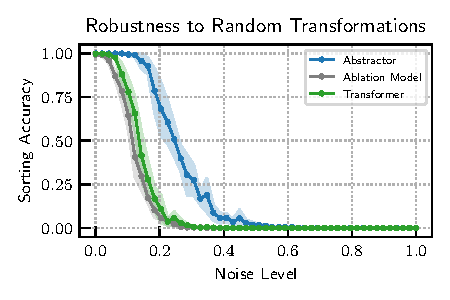
\includegraphics[scale=.95]{figures/experiments/additive_robustness.pdf}
        \vskip-5pt
        \caption{The Abstractor is more robust to corruption by additive noise. }\label{fig:exp_robustness1}
    \end{subfigure}\hspace{\fill}
    \begin{subfigure}[t]{0.40\textwidth}
        %\centering
        \hskip-.6in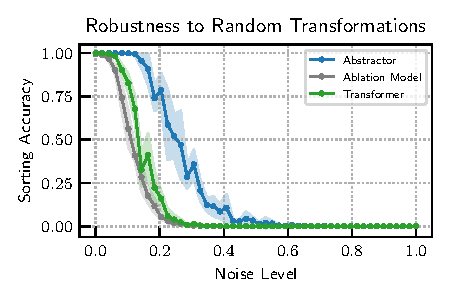
\includegraphics[scale=.95]{figures/experiments/multiplicative_robustness.pdf}
        \vskip-5pt
        \caption{The Abstractor is more robust to corruption by a random linear transformation.}\label{fig:exp_robustness2}
    \end{subfigure}
    \caption{Experiments on robustness.}\label{fig:exp_robustness}
\end{figure}